Latent semantic analysis (LSA) represents documents in a lower dimensional space called the latent semantic space by linear projection of term-document matrix through singular value decomposition. The term-document matrix represents the frequency of words from a pre defined vocbulary in a document. LSA has deficits like, capturing polysems and interpretation is difficult due to its unsatisfactory statiscal foundation. Probabilistic Latent Semantic Analysis (PLSA) introduces a statiscal foundation to LSA, since it is based on a liklihood principle and defines a generative model of document pertaining to the dataset ~\citep{Hofmann99probabilisticlatent}.

\begin{wrapfigure}{r}{0.40\textwidth}
\label{PLSM-genModel}
 \vspace{-20pt}
\begin{center}
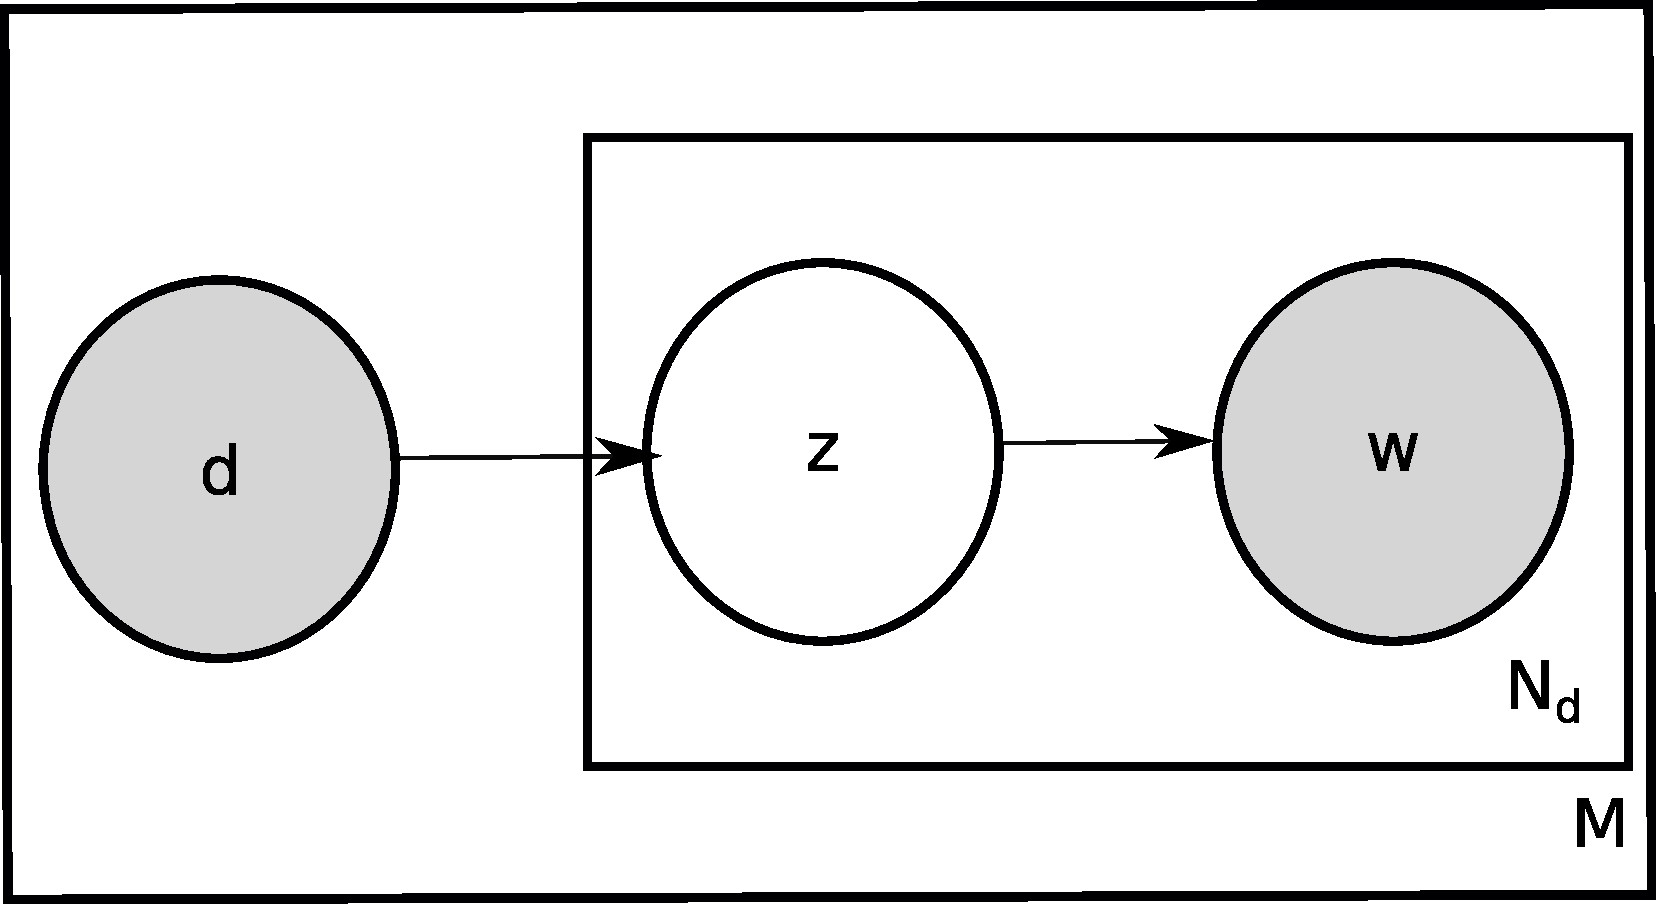
\includegraphics[width=0.38\textwidth]{PLSA}
\end{center}
 \vspace{-10pt}
 \caption{PLSA generative model: $d$ is the document variable, $z$ is the topic variable dependent on $d$ and $w$ is the word variable independent of $d$ given $z$. $d$ and $w$ are observed variables. $N_{d}$ is the document length and $M$ is the number of documents}
\vspace{-10pt}
\end{wrapfigure}
PLSA adopts the aspect model to model the joint probability of each co-occurrence of a word $ w ~\epsilon \ W = \{w_{1},w_{2}, \cdots , w_{V}\}$($V$ is the size of the vocabulary) in a document $ d ~\epsilon \ D = \{d_{1},d_{2}, \cdots , d_{M}\}$ by associating a latent class variable $z$. The generative process of the model in Fig. \ref{PLSM-genModel}  can be explained as below :

\begin{itemize}
\item[$\cdot$] pick a document $d$ with probability $P(d)$.
\item[$\cdot$] pick a topic with probability $P(z|d)$
\item[$\cdot$] pick a word from topic $z$ with probability $P(w|z)$
\end{itemize}

The above description joint probability model of PLSA is given by the expression:
\begin{eqnarray}
P(w,d) & = & P(d)\cdot P(w|d) \\
P(w|d) &= & \sum_{z}P(w|z)P(z|d)
\end{eqnarray}
PLSA is a mixture model. This is based upon the conditional independence assumption that given a topic, the choice of word is independent of the document. 

The parameters $P(z|d)$, $P(w|z)$ and $P(d)$ can be estimated by maximizing the log-liklihood function using the EM algorithm.
\begin{equation}
L = \sum_{d}\sum_{w}n(w,d)log(P(w,d)).
\end{equation}

The E-step can be obtained by using Baye's rule:
\begin{equation}
P(z|d,w) = \frac{P(z|d)\cdot P(w|z)}{\sum_{z}P(z|d)\cdot P(w|z)}
\end{equation}

By standard calculations, the equations for M-step can be obtained:
\begin{eqnarray}
P(z|d) & = & \frac{\sum_{w} n(w,d)P(z|w,d)}{\sum_{w}\sum_{z^{'}}n(w,d)P(z^{'}|w,d)} \\
P(w|z) & = & \frac{\sum_{d} n(w,d)P(z|w,d)}{\sum_{w}\sum_{d}n(w^{'},d)P(z|w{'},d)} \\
P(d) & = & \frac{\sum_{z}\sum_{w} n(w,d)P(z|w,d)}{\sum_{d^{'}}\sum_{w}\sum_{z}n(w,d^{'})P(z|w,d^{'})}
\end{eqnarray}



